\documentclass[oneside,english,12pt]{amsart}
\usepackage[T1]{fontenc}
\usepackage{amsmath, amsthm, amssymb, bm, bbm,soul}
\usepackage{url,color}
\usepackage{tikz}
\tikzset{
glow/.style={preaction={#1, draw, line join=round, line width=3pt, opacity=1}}
}

\begin{document}

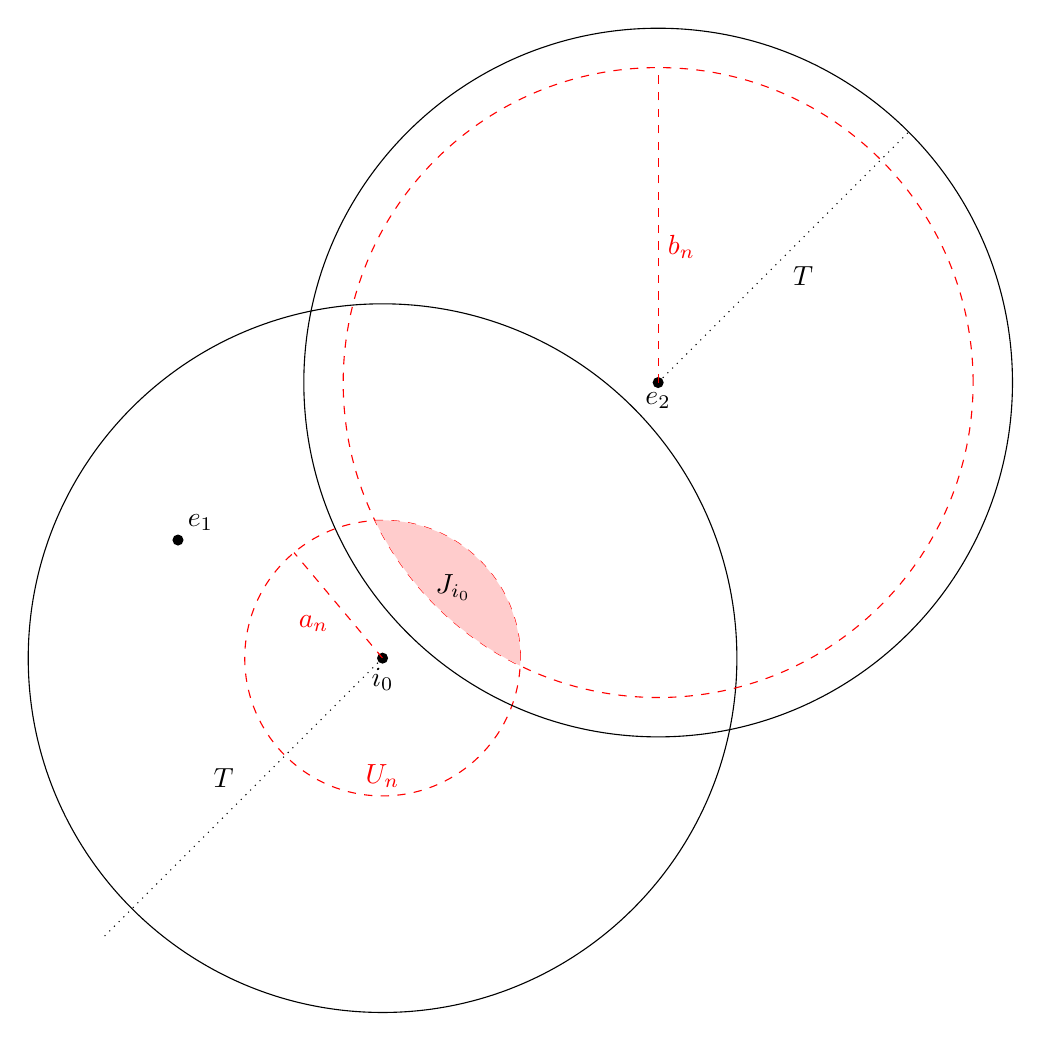
\begin{tikzpicture}
  % Draw the inner circle and label
  \draw[dashed,red] (0,0) circle (1.75cm);
  \fill (0,0) circle (2pt) node[below] {$i_0$};
  \draw[dashed,red] (0,0) -- node[midway, below left] {$a_n$} ++(130:1.75cm);
  
  % Draw a point inside the smaller circle and label
  \fill (150:3cm) circle (2pt) node[above right] {$e_1$};
  
  % Draw the larger circle and label
  \draw (0,0) circle (4.5cm);
  \draw[dotted] (0,0) -- node[midway, above left] {$T$} (-135:5cm);

  \draw (3.5,3.5) circle (4.5cm);
  \fill (3.5,3.5) circle (2pt) node[below] {$e_2$};
  \draw[dotted] (3.5,3.5) -- node[midway, below right] {$T$} ++(45:4.5cm);

  \draw[dashed,red] (3.5,3.5) circle (4cm);
  \draw[dashed,red] (3.5,3.5) -- node[midway, below right] {$b_n$} ++(90:4cm);


  % Fill the intersection
  \begin{scope}
    \clip (0,0) circle (1.75cm);
    \fill[red!20] (3.5,3.5) circle (4cm);
  \end{scope}

 
  \node[black] at (0.9, 0.9) {$J_{i_0}$};

  % Label the small red circle
  \node[red] at (0,-1.5) {$U_n$};
\end{tikzpicture}

\end{document}